\newpage
\usecaseristoratore{Assegnamento ingredienti ad un piatto}
\label{usecase:Assegnamento ingredienti ad un piatto}

\begin{figure}[h]
	\centering
	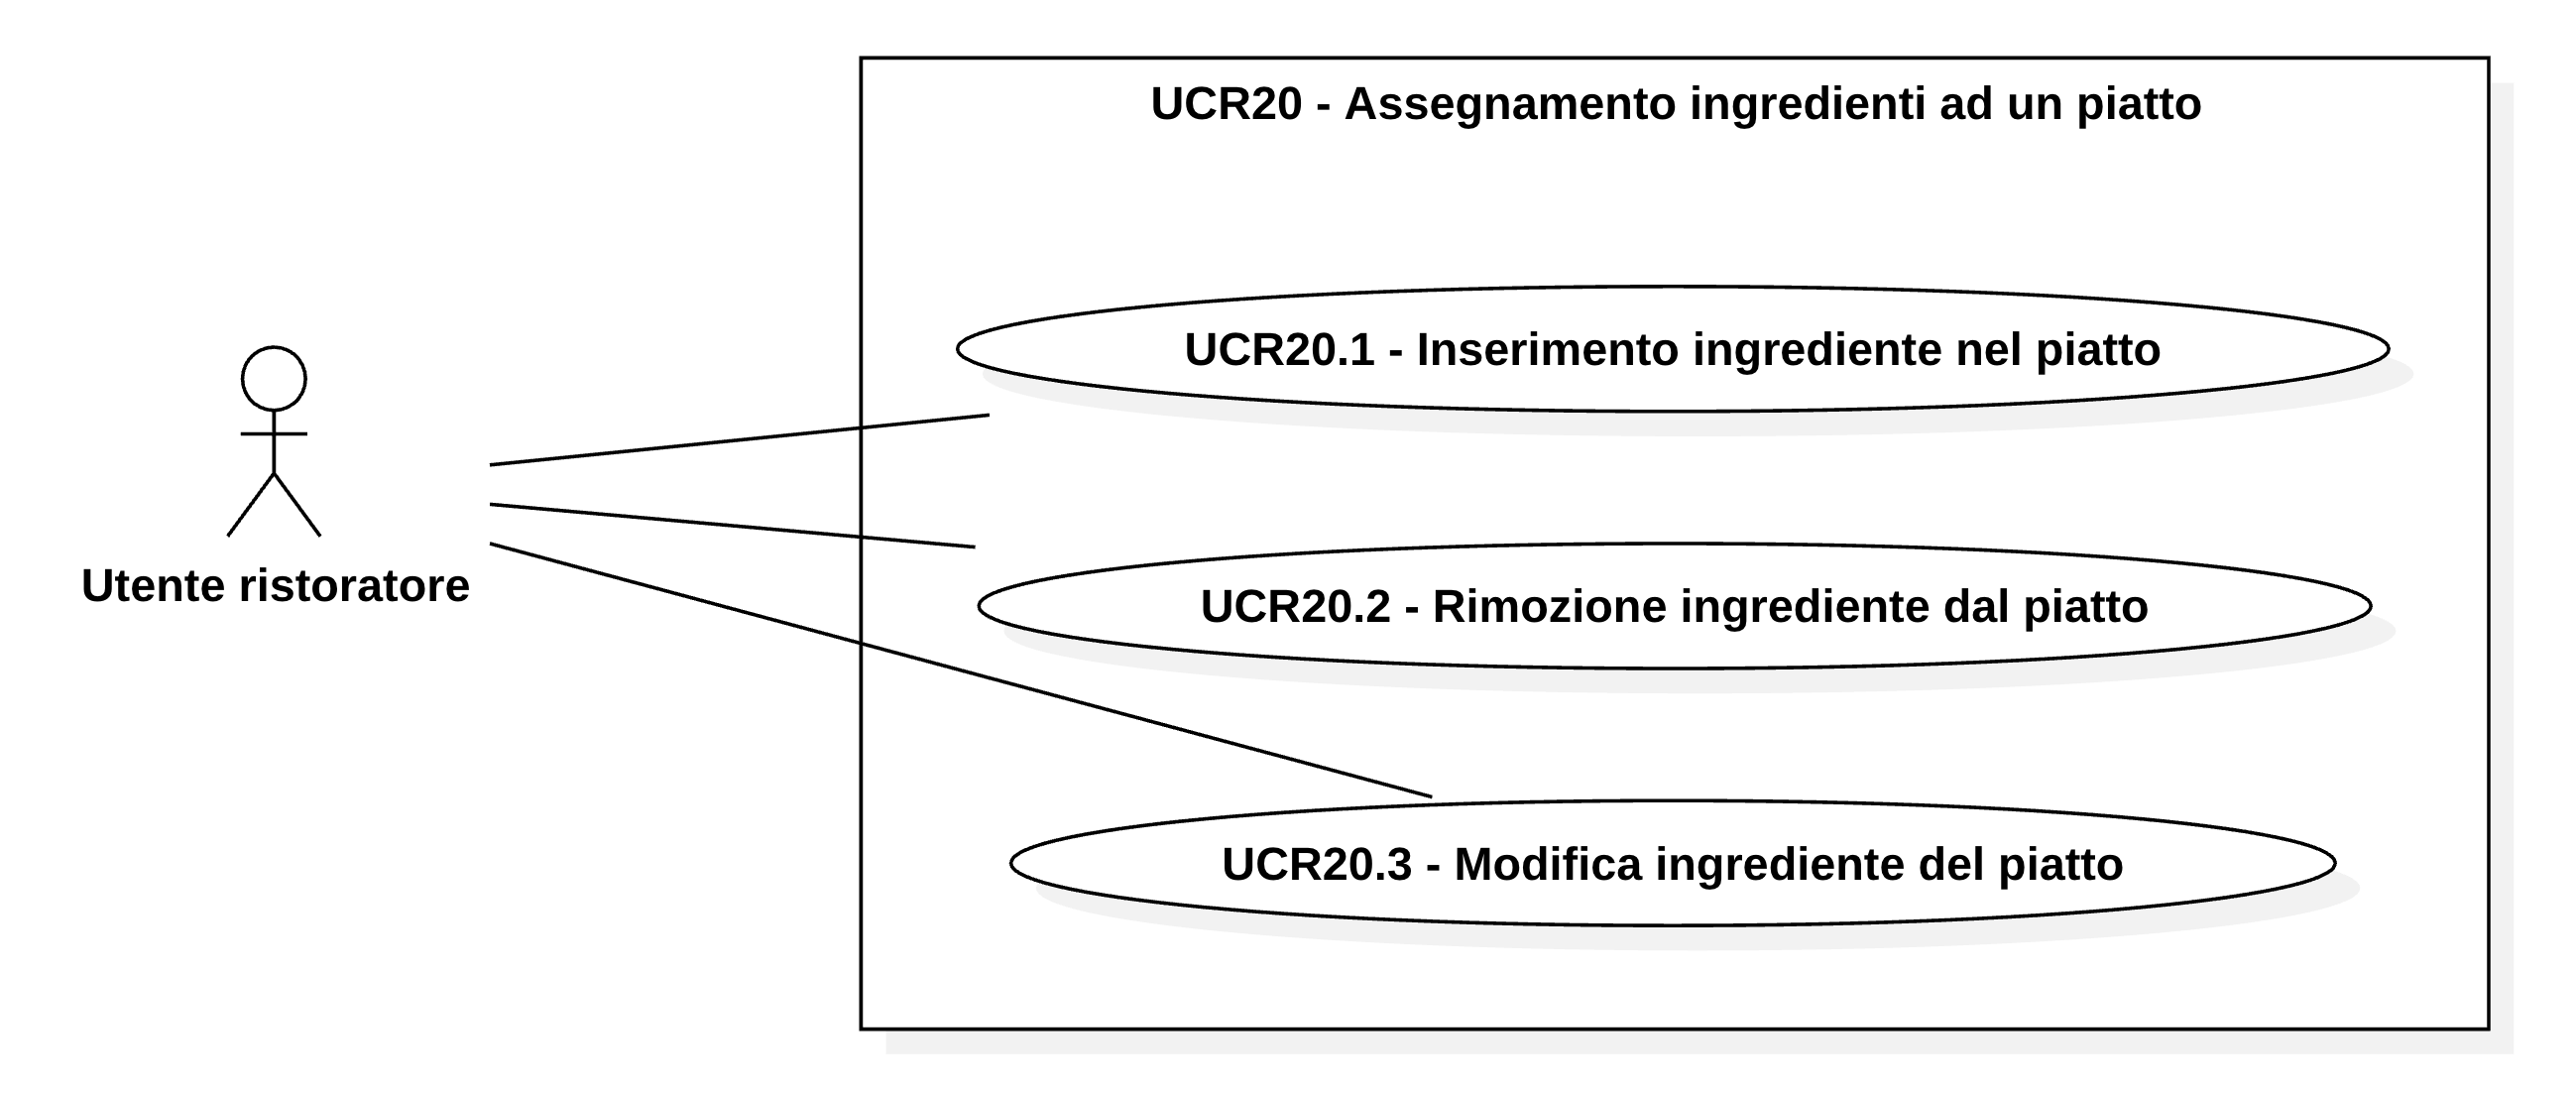
\includegraphics[width=0.9\textwidth]{./uml/UCR20.png} 
	\caption{Assegnamento ingredienti ad un piatto}
	\label{fig:UCR20}
  \end{figure}

\begin{itemize}
	\item \textbf{Attore principale:} Utente ristoratore.

	\item \textbf{Precondizione:} L'Utente ristoratore ha effettuato l'accesso al Sistema (vedi \autoref{usecase:Effettua accesso}).


	\item \textbf{Postcondizione:}
	      L'Utente ristoratore ha assegnato tutti gli ingredienti ad un piatto.

	\item \textbf{Scenario principale:}
	      \begin{enumerate}
		      \item L'Utente ristoratore assegna tutti gli ingredienti necessari ad un piatto;

		      \item Il Sistema registra gli ingredienti assegnati ad un piatto.
        \end{enumerate}
\end{itemize}
